\section{Confronto del modello di coalescenza con il CSM}
In questa sezione si esegue un confronto tra il modello di coalescenza e il modello di adronizzazione statistica canonica.
Per far ciò confrontiamo i modelli teorici con dati sperimentali riguardo alle misure di rapporti di produzione tra nuclei e protoni in funzione della molteplicità \cite{alice_2022_coal_formula}.
Più specificatamente si vanno a considerare i rapporti $(D+\bar D)/(p + \bar p)$ e $(^3\text{He} + ^3\overline{\text{He}})/(p+\bar p)$.
I grafici prodotti sono riportati in \autoref{fig:NoPvsMult}.
Per le previsioni del CSM utilizza il pacchetto software del \ttbox{Thermal-FIST} \cite{Vovchenko_2019_thermal_FIST}, utilizzando dei volumi di correlazione $V_C$ tra 1 e 3 unità di rapidità.
Invece, per il modello di coalescenza si utilizza l'implementazione effettuata in \cite{Sun_2019_coal_model}.
È importante notare che si sono utilizzati due modelli di coalescenza per il nucleo di (anti)$^{3}{\rm He}$: il modello di coalescenza a tre corpi, in cui si assume la formazione del nucleo a partire dalla vicinanza di due protoni e di un neutrone; il modello a due corpi, in cui si assume la formazione del nucleo a partire da un (anti)deuterone e un (anti)neutrone. 
\begin{figure}[h]
    \centering
    \begin{subfigure}{.49\textwidth}
    \centering
        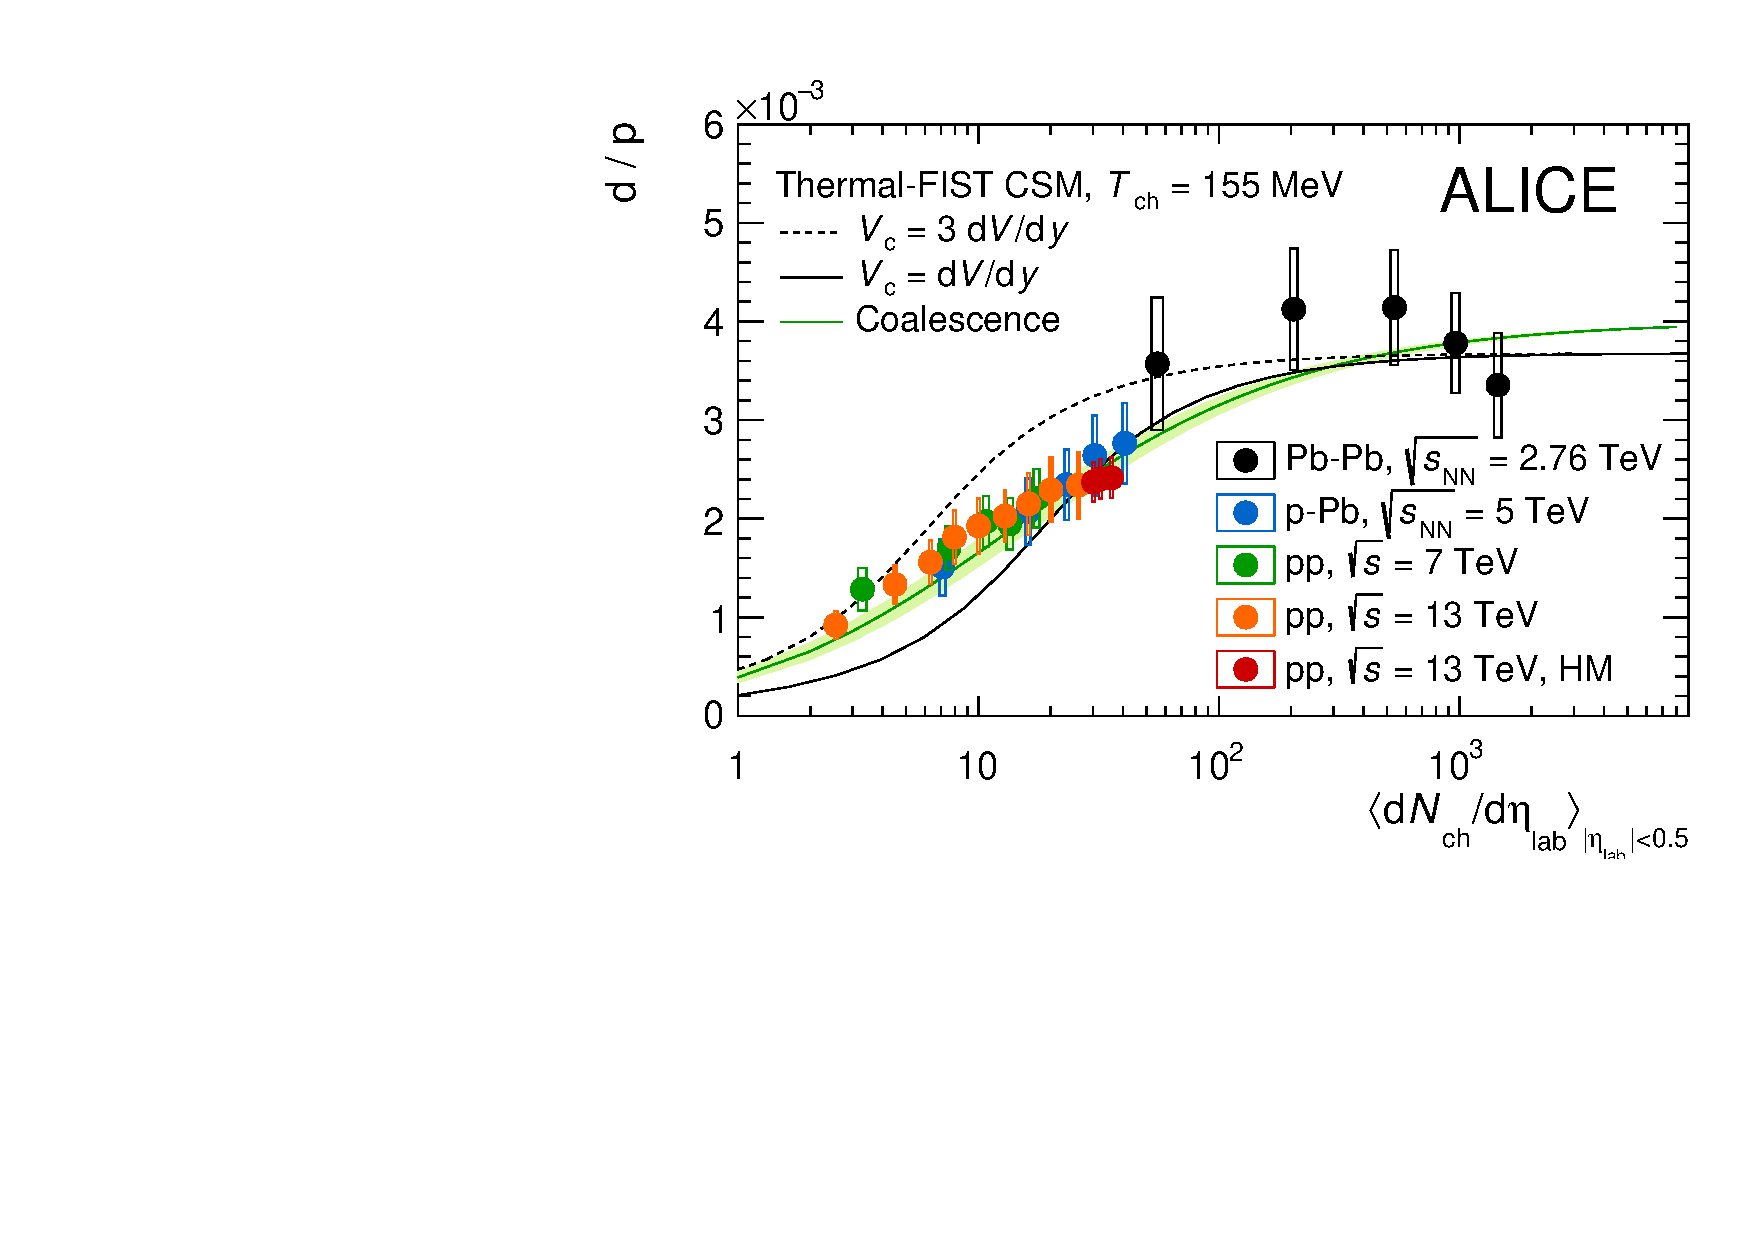
\includegraphics[width=\textwidth]{image/2-modelli/cDoPvsMult.pdf}
        \caption{$(D+\bar D)/(p + \bar p)$}
        \label{fig:cDoPvsMult}
    \end{subfigure}
    %\hspace{1cm}
    \begin{subfigure}{.49\textwidth}
        \centering
        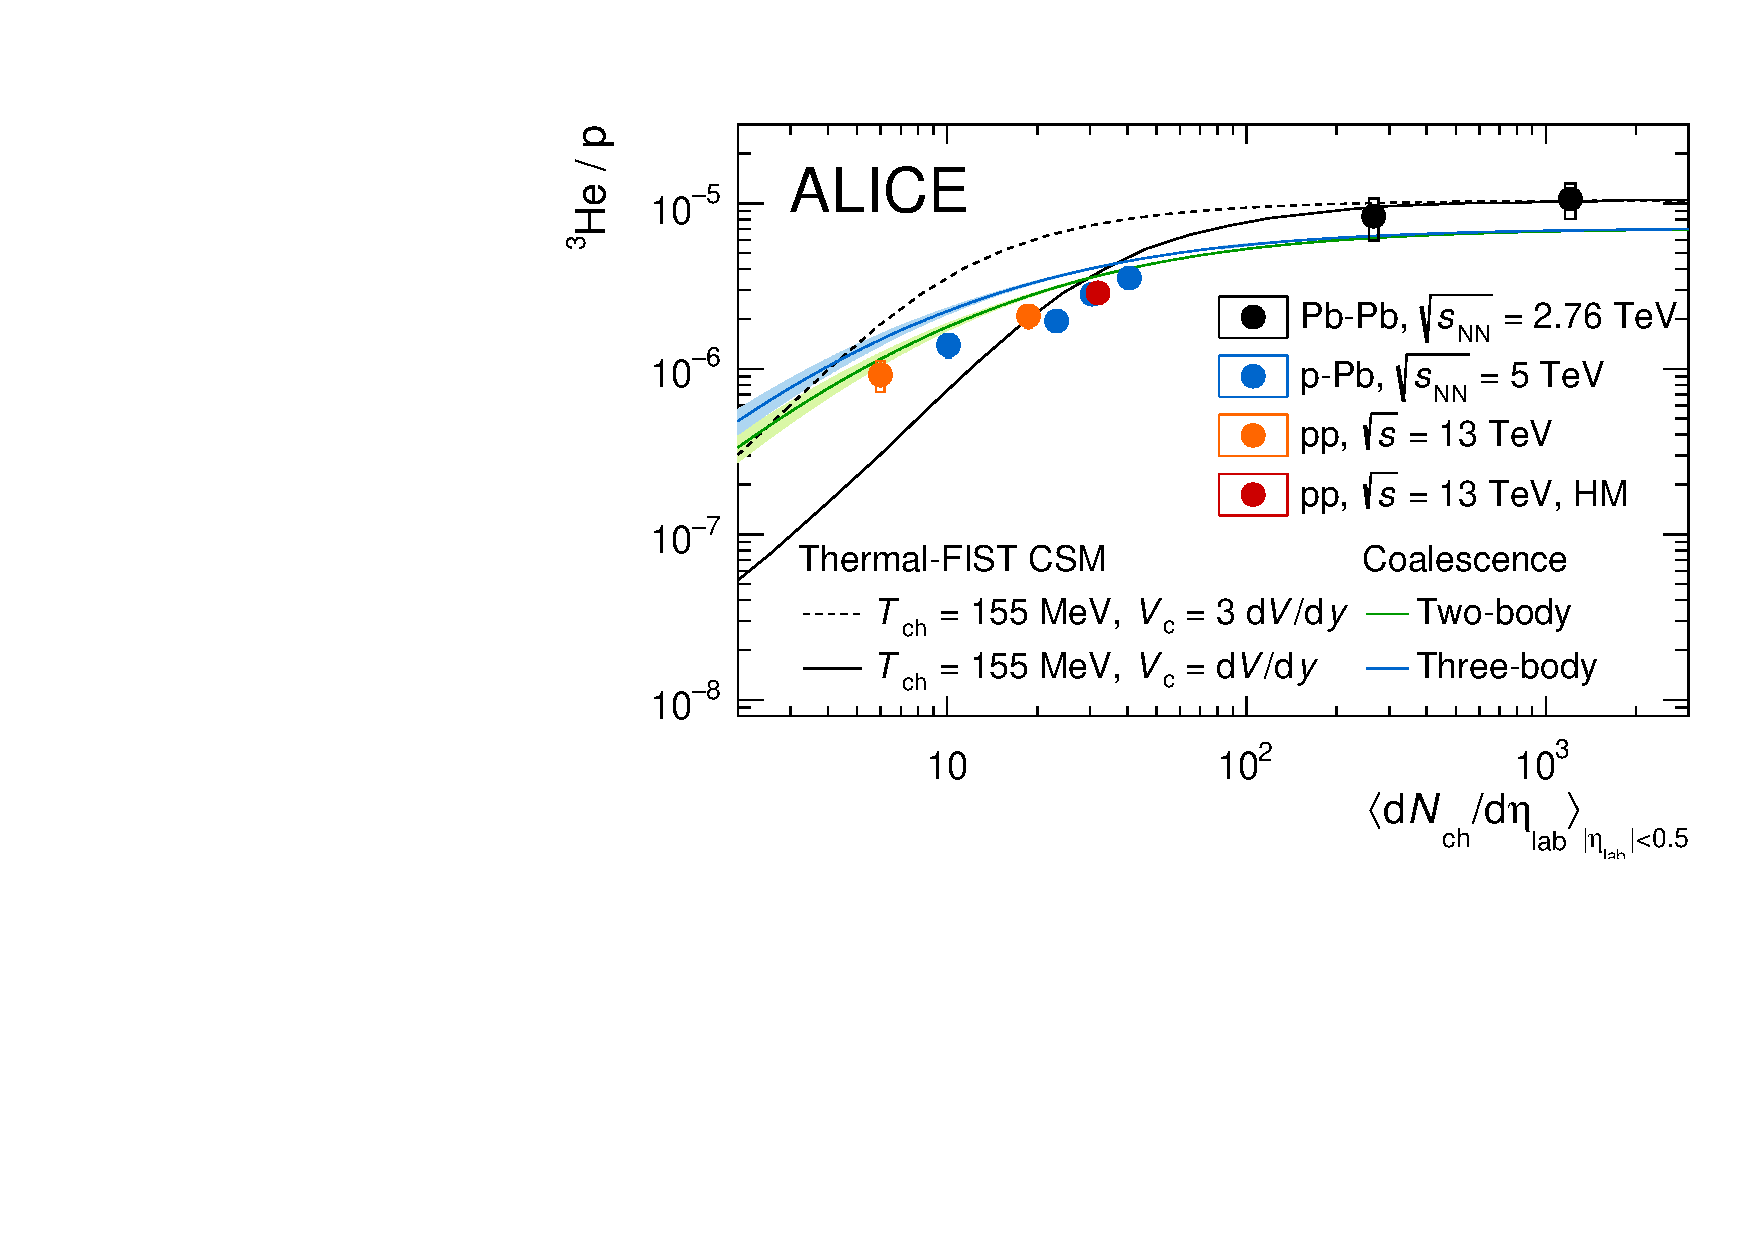
\includegraphics[width=\textwidth]{image/2-modelli/cHEoPvsMult.pdf}
        \caption{$(^3\text{He} + ^3\overline{\text{He}})/(p+\bar p)$}
        \label{fig:cHEoPvsMult}
    \end{subfigure}
    \captionwithsource{Misure (punti colorati) dei rapporti tra la produzione dei nuclei e protoni in funzione della molteplicità per \emph{\rmfamily (a)} (anti)deuteroni e \emph{\rmfamily (b)} (anti)nuclei di $^3\text{He}$. Le linee nere continue e tratteggiate rappresentano le previsioni del \emph{\ttbox{Thermal-FIST}} CSM.
    "$d/p$" indica $(D+\bar D)/(p + \bar p)$ e "$^3\text{He}/p$" indica $(^3\text{He} + ^3\overline{\text{He}})/(p+\bar p)$.
    In \emph{\rmfamily (a)} la linea verde rappresenta il modello di coalescenza, in \emph{\rmfamily (b)} la linea verde e blu rappresentano rispettivamente il modello di coalescenza a due corpi e a tre corpi.}{\cite{alice_2022_coal_formula}} 
    \label{fig:NoPvsMult}
\end{figure}

Per quanto riguarda le misure sperimentali, esse sono consistenti con esperimenti effettuati in passato \cite{Adam_2016_a1, 2017_a2, Acharya_2018_a3}: gli andamenti dei due rapporti aumentano con l'aumentare della molteplicità e i valori si saturano ad alte molteplicità.
Per quanto riguarda invece le previsioni teoriche, solamente il modello di coalescenza sembra essere qualitativamente in accordo con i dati, per entrambi i rapporti.
In particolare per $D/p$, il modello di coalescenza riesce a riprodurre fedelmente i dati per tutto l'intervallo della molteplicità, mentre per $^3\text{He}$ abbiamo una migliore concordanza del modello di coalescenza a due corpi nelle regioni a bassa bassa molteplicità, mentre ad alte molteplicità (come per le misure delle collisioni Pb-Pb) si ha un discostamento maggiore.
Il modello statistico canonico fornisce invece un andamento più qualitativo per molteplicità più basse, mentre ha un andamento consistente con i dati nel regime del gran-canonico (ossia nelle molteplicità caratterizzate dagli urti Pb-Pb).